\section{需求分析}

本程序要完成的功能为,判断字符串是否为回文字符串。
输入要求是一串字符串,并且要以\#结束。
例如,
avava\#。
如果有必要,可以读入多个字符串串。
ava\#abaaba\#asd88\#。
我们对输入做出以下限制:
\begin{enumerate}
   \item 输入的串的总长度不能超过$10^6$
   \item 输入的所有字符只能在[0~9][a~z][A~Z]中\#
\end{enumerate}


在正常情况下,本程序输出T或F判断正误。在有多个字符串输入的情况下,
判断结果将按顺序输出。
以上面两个输入样例为例。

Match


Match Match Dismatch



\section{概要设计}
   主程序,即在main函数中调用输入和创建初始化数据结构的函数,进行数据处理,最后输出
   结果。


   我们需要定义以下数据结构
   \begin{enumerate}
      \item 队列,只需要支持队列的基本操作
      \item 栈,只需要支持栈的基本操作
      \item 处理数据的solution
   \end{enumerate}


   对于读入非\#字符,main会调用Solution中的insert函数插入数据。
   每当读入一个\#的时候,main中就会调用Solution中check函数判断之前读入的串是否为回文串。

\newpage

\section{详细设计}
   \begin{figure}[H]
      \centering
      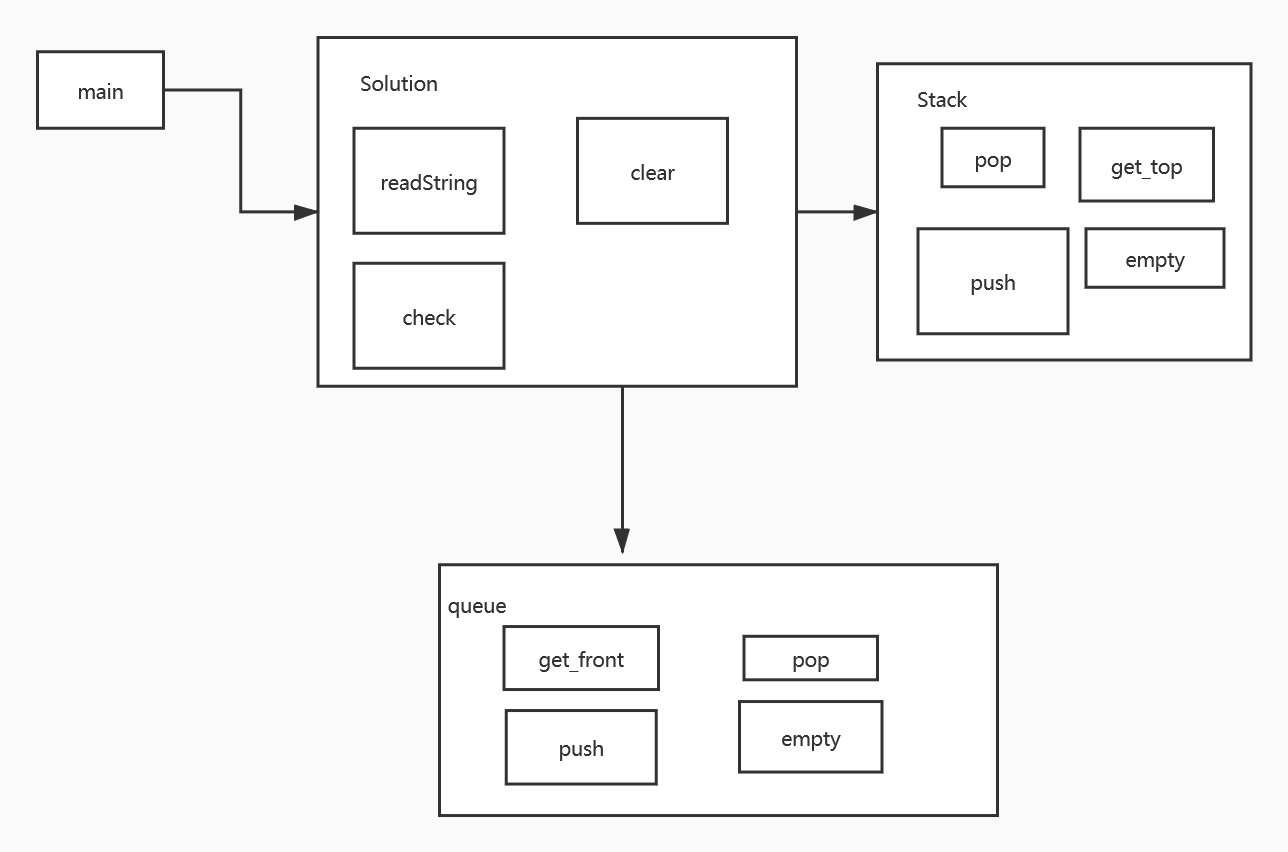
\includegraphics[width=0.5\textwidth]{images/process.jpg}
      \caption{函数调用关系图}
   \end{figure}

   先分别定义队列和栈数据结构


   队列中含有的元素为:
   \begin{enumerate}
      \item 头指针,head
      \item 尾指针,tail
      \item 插入insert
      \item 弹出数据pop\_tail
      \item 获取数据get\_head
   \end{enumerate}


   同样有栈的定义如下
   \begin{enumerate}
      \item 栈顶指针top
      \item 取得栈顶的数据get\_top
      \item 弹出栈顶的数据pop\_top
   \end{enumerate}

\newpage

\begin{algorithm}[htb] 
   \caption{ Solution结构定义 } 
   \label{alg:Framwork} 
   \begin{algorithmic}[1]
      \Require 输入串
      \Ensure 判断串是否回文
      
      \State 插入数据函数
      \Function {insert}{a}
         \If {a 不合法}
            \State \Return FAILURE
         \EndIf
         \State 将a添加到栈中
         \State 将a添加到队列中
         \State \Return SUCCESS
      \EndFunction \\

      \State 检查是否为回文串函数
      \Function {check}{void}
         \While{栈和队列非空}
            \State 从栈中取出一个元素stack\_data
            \State 从队列中取出一个元素queue\_data
            \If{$stack\_dat \neq queue\_data$}
               \State \Return FAILURE
            \EndIf
            \State 从栈和队列中弹出数据
         \EndWhile
         \State \Return SUCCESS
      \EndFunction
   \end{algorithmic} 
   \end{algorithm}

\newpage

\section{调试分析报告}

   我们在这里复用了实验二的stack.h

在使用线性数据结构的操作下,算法复杂度几乎已经达到了下界,即$O(N)$。
   但是空间复杂度上面还有许多可以优化的地方。我们人为定义的数据上限为$10^6$。但是显然,
   在大多数情况下用户使用的空间会远远低于这个上界。所以一次申请$10^6$显然是过度浪费内存的。


   所以我们将栈的数据存储到一个叫做Vector的动态数组中,这个数组开始时数据边界为$10^2$级别。
   在使用过程中,这个数组会自动调用$resize()$扩大边界。我们设一个系数$k$,每次$resize()$后的边界为原来的$k$倍。
   接下来我们将测试不同$k$下由$resize$造成的浪费。



% Please add the following required packages to your document preamble:
% \usepackage{booktabs}
% \usepackage{longtable}
% Note: It may be necessary to compile the document several times to get a multi-page table to line up properly
\begin{longtable}[c]{@{}lllll@{}}
   \toprule
   N   & $10^4$ & $10^5$ & $10^6$ &  \\* \midrule
   \endfirsthead
   %
   \endhead
   %
   \bottomrule
   \endfoot
   %
   \endlastfoot
   %
   1.6 & 29634  & 121688 & 121688 &  \\
   2.0 & 32704  & 65472  & 65472  &  \\
   2.4 & 20807  & 120056 & 120056 &  \\* \bottomrule
   \end{longtable}


   观察发现,在$k=1.6$与$k=2.4$时,数据表现较为极端,而$k=2.0$时较为平稳,所以我们选择$k=2.0$作为我们的vector的resize系数。


\newpage

\section{用户使用说明}
   用户可以使用IDE或者手动编译源代码stack.cpp,获得可执行文件。

   笔者使用的gcc版本为8.1.0
   运行可执行文件后,用户可以选择文件输入或者交互式输入。
   在文件输入下输出将会从定向到output.in。
   结束程序可以输入EOF

\section{测试结果}

   我们使用我们手工构造的数据
   ava\#abaaba\#asd88\#

   根据程序输出,我们判断手工与程序输出相同。
   即通过测试。



